\textbf{Цель работы:} Подтверждение закона Бойля-Мариотта.

\textbf{Оборудование:} Установка для демонстации закона Бойля-Мариотта (рис.\ref{fig:установка для демнострации закона Бойля-Мариотта})

\begin{figure}[!h]
    \centering
    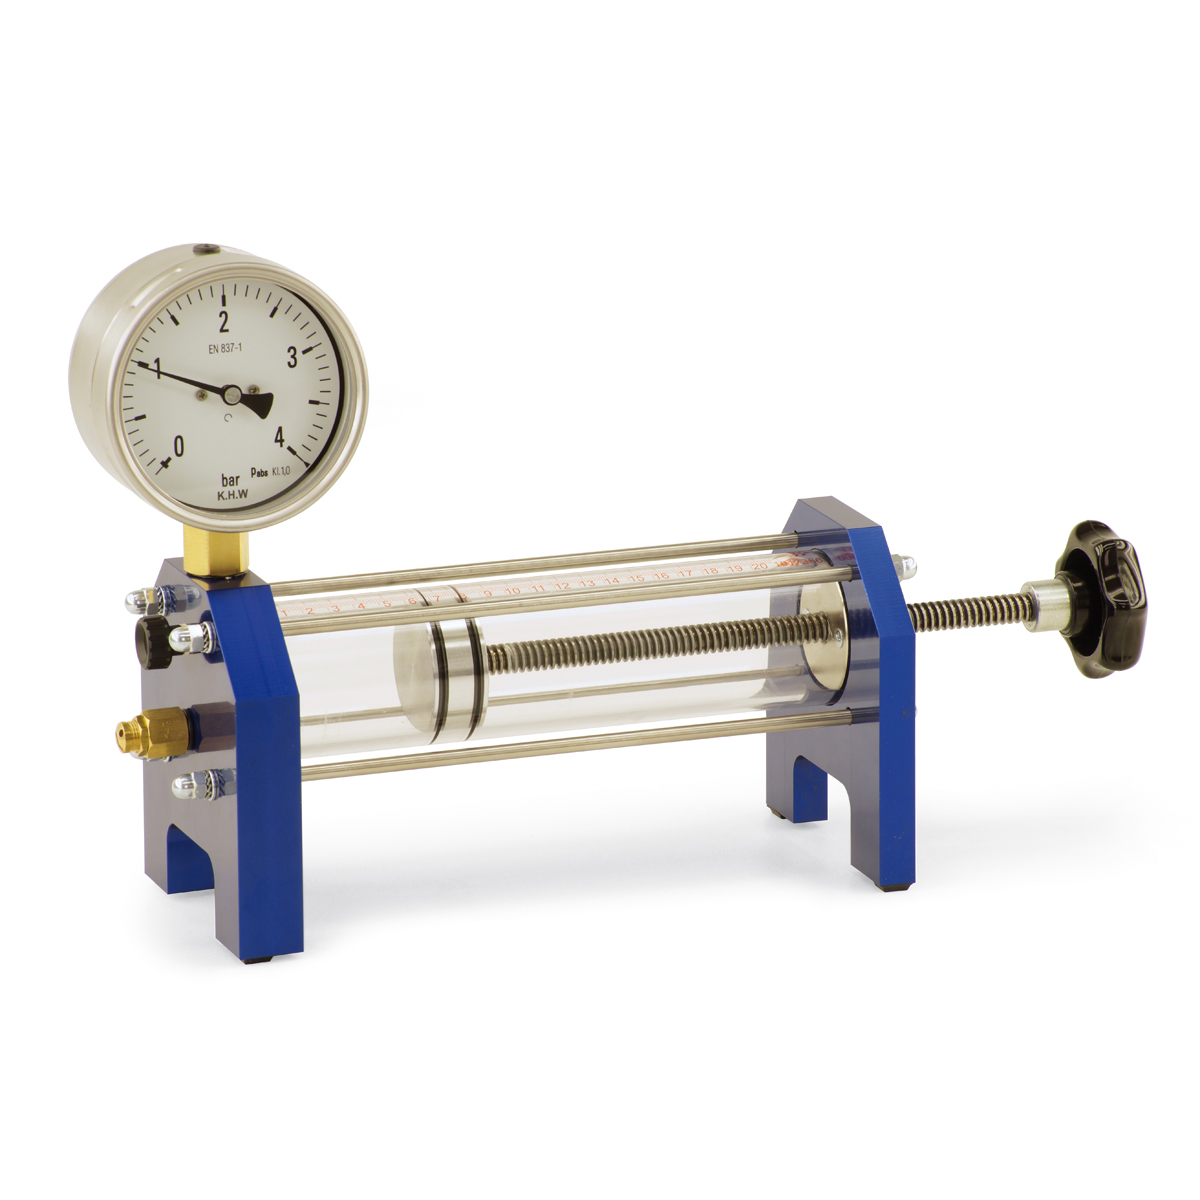
\includegraphics[width = 0.3\textwidth]{image/image2.png}
    
    \caption{Установка для демонстации закона Бойля-Мариотта}
    
    \label{fig:установка для демнострации закона Бойля-Мариотта}
\end{figure}

\textbf{Ход работы:}

\begin{enumerate}
    \item{Открыли запорный вентиль на левой опоре установки.}
    \item{Установили поршень внутри прозрачноо цилиндра в положение $S_0 = 20 ~ \text{см}$ и закрыли вентиль.}
    \item{Сняли показание давления и записли в таблицу \ref{tab:main_tab}.}
    \item{Изменяли положение поршня по 1"=му см. В каждом положении снимали и записывали показания давления в цилиндре}
    \item{Установили поршень в положение $S_0$, открыли вентиль, сбросив давление, и закрыли.}
    \item{Затем установили поршень в положение $S = 20$. Изменяли положение поршня пошагово по 1"=му см. В каждом положении снимали и регистрировали показания давления.}
    \item{Установили поршень в положение $S_0 = 5$, открыли вентиль сбросив давление, и закрыли.}
    \item{Затем установили поршень в положение $S = 20$. Изменяли положение поршня пошагово по 1"=му см. В каждом положении давления.}
    \item{Расчитали объем воздуха $V$, находящегося в закрытом пространстве цилиндра лаборатоной установки по данным о расстоянии $S$, на котором находится поршень по отношению к положению нулевого объема и площади поперечного сечения A поршня.}
    \item{Рассчитали при помощи уравнения $p V = \nu R T$, (где $T$ "--- температура газа, $R$ "--- универсальная газовая постоянная, $\nu$ "--- количество вещества) количество вещества в цилиндре, выраженное в молях}
    
    $
        \nu_1 = \frac{565.49}{8.314 \cdot 293.15} \approx 23.2 \text{мМоль}
    $
    
    $
        \nu_2 \approx 46.4 \text{мМоль}
    $
    
    $
        \nu_3 \approx 92.81 \text{мМоль}
    $
    \item{Построили графики зависимости $P$ от $V$ (рис.\ref{graph:main_graph})}
\end{enumerate}

\textbf{Эксперементальные данные:}

Эксперементальные данные представленны в таблице \ref{tab:main_tab}
\begin{table}[H]
    \centering
    \begin{tabular}{|c|c|c|c|c|}
        \hline
        \makecell{Положение \\ поршня $S$, см} & 
        \makecell{Рабочий объем \\ цилиндра $V \text{, см}^3$} &
        \multicolumn{3}{|c|}{\makecell{Давление воздуха при различном \\ его количестве в рабочем объеме \\ цилиндра $p$, бар}} \\
        \cline{3-5}
        & & {$S_0 = 20$} & {$S_0 = 10$} & {$S_0 = 5$}\\ 
        \hline 
        1 & 113.09 & - & - & 3 \\
        \hline 
        2 & 226.19 & - & 3.84 & 2.12 \\
        \hline 
        3 & 339.29 & - & 2.9 & 1.55 \\
        \hline 
        4 & 452.39 & - & 2.29 & 1.22 \\
        \hline 
        5 & 565.49 & 3.63 & 1.9 & 1 \\
        \hline 
        6 & 678.58 & 3.09 & 1.61 & 0.85 \\
        \hline 
        7 & 791.68 & 2.7 & 1.4 & 0.73 \\
        \hline 
        8 & 904.78 & 2.4 & 1.23 & 0.65 \\
        \hline 
        9 & 1017.9 & 2.15 & 1.1 & 0.58 \\
        \hline 
        10 & 1130.97 & 1.95 & 1 & 0.5 \\
        \hline 
        11 & 1244.1 & 1.79 & 0.91 & 0.47 \\
        \hline 
        12 & 1357.2 & 1.64 & 0.84 & 0.43 \\
        \hline 
        13 & 1470.3 & 1.51 & 0.78 & 0.4 \\
        \hline 
        14 & 1583.4 & 1.4 & 0.71 & 0.36 \\
        \hline 
        15 & 1696.5 & 1.31 & 0.67 & 0.35 \\
        \hline 
        16 & 1809.6 & 1.22 & 0.62 & 0.33 \\
        \hline 
        17 & 1922.7 & 1.18 & 0.59 & 0.3 \\
        \hline 
        18 & 2035.8 & 1.1 & 0.55 & 0.28 \\
        \hline 
        19 & 2148.8 & 1.05 & 0.52 & 0.26 \\
        \hline 
        20 & 2261.9 & 1 & 0.5 & 0.25 \\
        \hline
\end{tabular}
\caption{Эксперементальныйе данные}
\label{tab:main_tab}
\end{table}

Вывод:

В лабораторной работе мы проверили закон Бойля"=Мариотта, измерили давление воздуха при постоянном количестве вещества и температуре, передвигая поршень, и построили графики зависимости давления от объёма. Закон Бойля"=Мариотта действует, т.к. для всех измеренных значений $p V = const$ построенные графики гиперболические, что так же подтверждает закон

\begin{figure}[!h]
\begin{center}
\begin{tikzpicture}
    \begin{axis}
        [
            width=\linewidth, % Scale the plot to \linewidth 
            legend pos = north east,
            xlabel=$V ~ \text{см}^3$, % Set the labels
            ylabel=$p ~ \text{бар}$,
            ymin = 0,
            xmin = 0,
            grid = major
        ]
        \addplot table[x=column 1,y=column 2,col sep=comma] {csvTable/table1.csv}; 
        \addplot table[x=column 1,y=column 2,col sep=comma] {csvTable/table2.csv};
        \addplot table[x=column 1,y=column 2,col sep=comma] {csvTable/table3.csv};
        \legend{
            $S_0 = 20$,
            $S_0 = 10$,
            $S_0 = 5$,
        };
      \end{axis}
    \end{tikzpicture}
  \end{center}
\caption{График зависимости $P$ от $V$}
\label{graph:main_graph}
\end{figure}
